\documentclass[11pt,a4paper]{article}

\usepackage[utf8]{inputenc}
\usepackage[T1]{fontenc}

\usepackage[spanish]{babel}
\decimalpoint
\addto\captionsspanish{
  \renewcommand{\tablename}{Tabla}
}

\usepackage{csquotes}
\usepackage{lmodern}

% Maths
\usepackage{amsmath, amsfonts, amssymb, amsthm}
\usepackage{siunitx}

% Graphs
\usepackage{graphicx}
\usepackage{float}
\usepackage{subcaption}

% Code (python)
\usepackage[newfloat]{minted}
\usemintedstyle{friendly}
\SetupFloatingEnvironment{listing}{name=Código}

% Format
\usepackage[margin=2.5cm]{geometry}
\usepackage{fancyhdr}
\usepackage{booktabs}
\setlength{\parindent}{0pt}
\setlength{\parskip}{0.5em}

% Bibliography
\usepackage[backend=biber, style=ieee]{biblatex}
\addbibresource{bibliography/refs.bib}

% Links and references
\usepackage{hyperref}
\hypersetup{
  colorlinks=true,
  linkcolor=black,
  filecolor=magenta,
  urlcolor=cyan,
  citecolor=black,
  pdftitle={Trabajo Grupal - Primer Parcial - Física Computacional}
}

% Heads
\pagestyle{fancy}
\fancyhf{}
\lhead{\textbf{Física Computacional}}
\rhead{Trabajo Grupal - Primer Parcial}
\cfoot{\thepage}
\renewcommand{\headrulewidth}{0.4pt}

% Portada information
\title{
    \vspace{-1.5cm}
    \rule{\textwidth}{1pt}\\[0.5cm]
    \textbf{\huge Trabajo Grupal - Primer Parcial}\\[0.3cm]
    \Large Física Computacional
    \vspace{0.2cm}
    \rule{\textwidth}{1pt}
}
\author{
  \textbf{Nombres de los Integrantes:} \\
  Mamani Huarsaya, Jorge Luis \\
  Estudiante 2 \\
  Estudiante 3
}
\date{\today}

\begin{document}

% Portada
\maketitle
\thispagestyle{empty}
\newpage

% Index
\tableofcontents
\newpage

% Sections
\section{Movimiento parabólico}

\subsection{Enunciado}
La trayectoria de una partícula es (extraído del libro de Serway o Sears):
\begin{equation}
    y = x \tan \alpha_0 - \frac{g}{2v_0^2 \cos^2 \alpha_0} x^2
    \label{eq:mov_parabolico}
\end{equation}
donde $v_0$ y $\alpha_0$ son las condiciones iniciales.

\begin{enumerate}
    \item Mediante una gráfica determine el alcance mediante la ecuación de arriba. Las condiciones iniciales son $v_0 = \SI{5}{\meter/\second}$ con $\alpha_0 = 60^\circ$.
    \item Aplicar el método de Heun y encuentre el alcance.
    \item Haga la comparación de los resultados encontrados. Para ello varíe el tamaño de paso $h$ para que el resultado sea confiable.
\end{enumerate}

\subsection{Aplicación de la ecuación}

Para resolver la primera parte del problema, se utilizó directamente la ecuación analítica del movimiento parabólico mostrada en la Ecuación \ref{eq:mov_parabolico}. Se implementó un programa en Python que genera múltiples valores de la posición horizontal $x$ y evalúa la altura correspondiente $y(x)$ para cada punto.

Las condiciones iniciales consideradas fueron $v_0 = \SI{5}{\meter/\second}$, $\alpha_0 = 60^\circ$ y $g = \SI{10}{\meter/\second^2}$. Luego, se graficó la trayectoria de la partícula y se observó la forma parabólica característica del movimiento y determinar visualmente el alcance horizontal.

La implementación utilizada se muestra en el Código \ref{lst:prob1_1}.

\begin{listing}[H]
\inputminted[
    linenos,
    frame=lines,
    mathescape,
    fontsize=\small
]{python}{code/problem01_1.py}
\caption{Implementación de la gráfica de la ecuación \ref{eq:mov_parabolico}.}
\label{lst:prob1_1}
\end{listing}

La Figura \ref{fig:prob1} muestra la trayectoria obtenida mediante la ecuación analítica.

\begin{figure}[H]
  \centering
  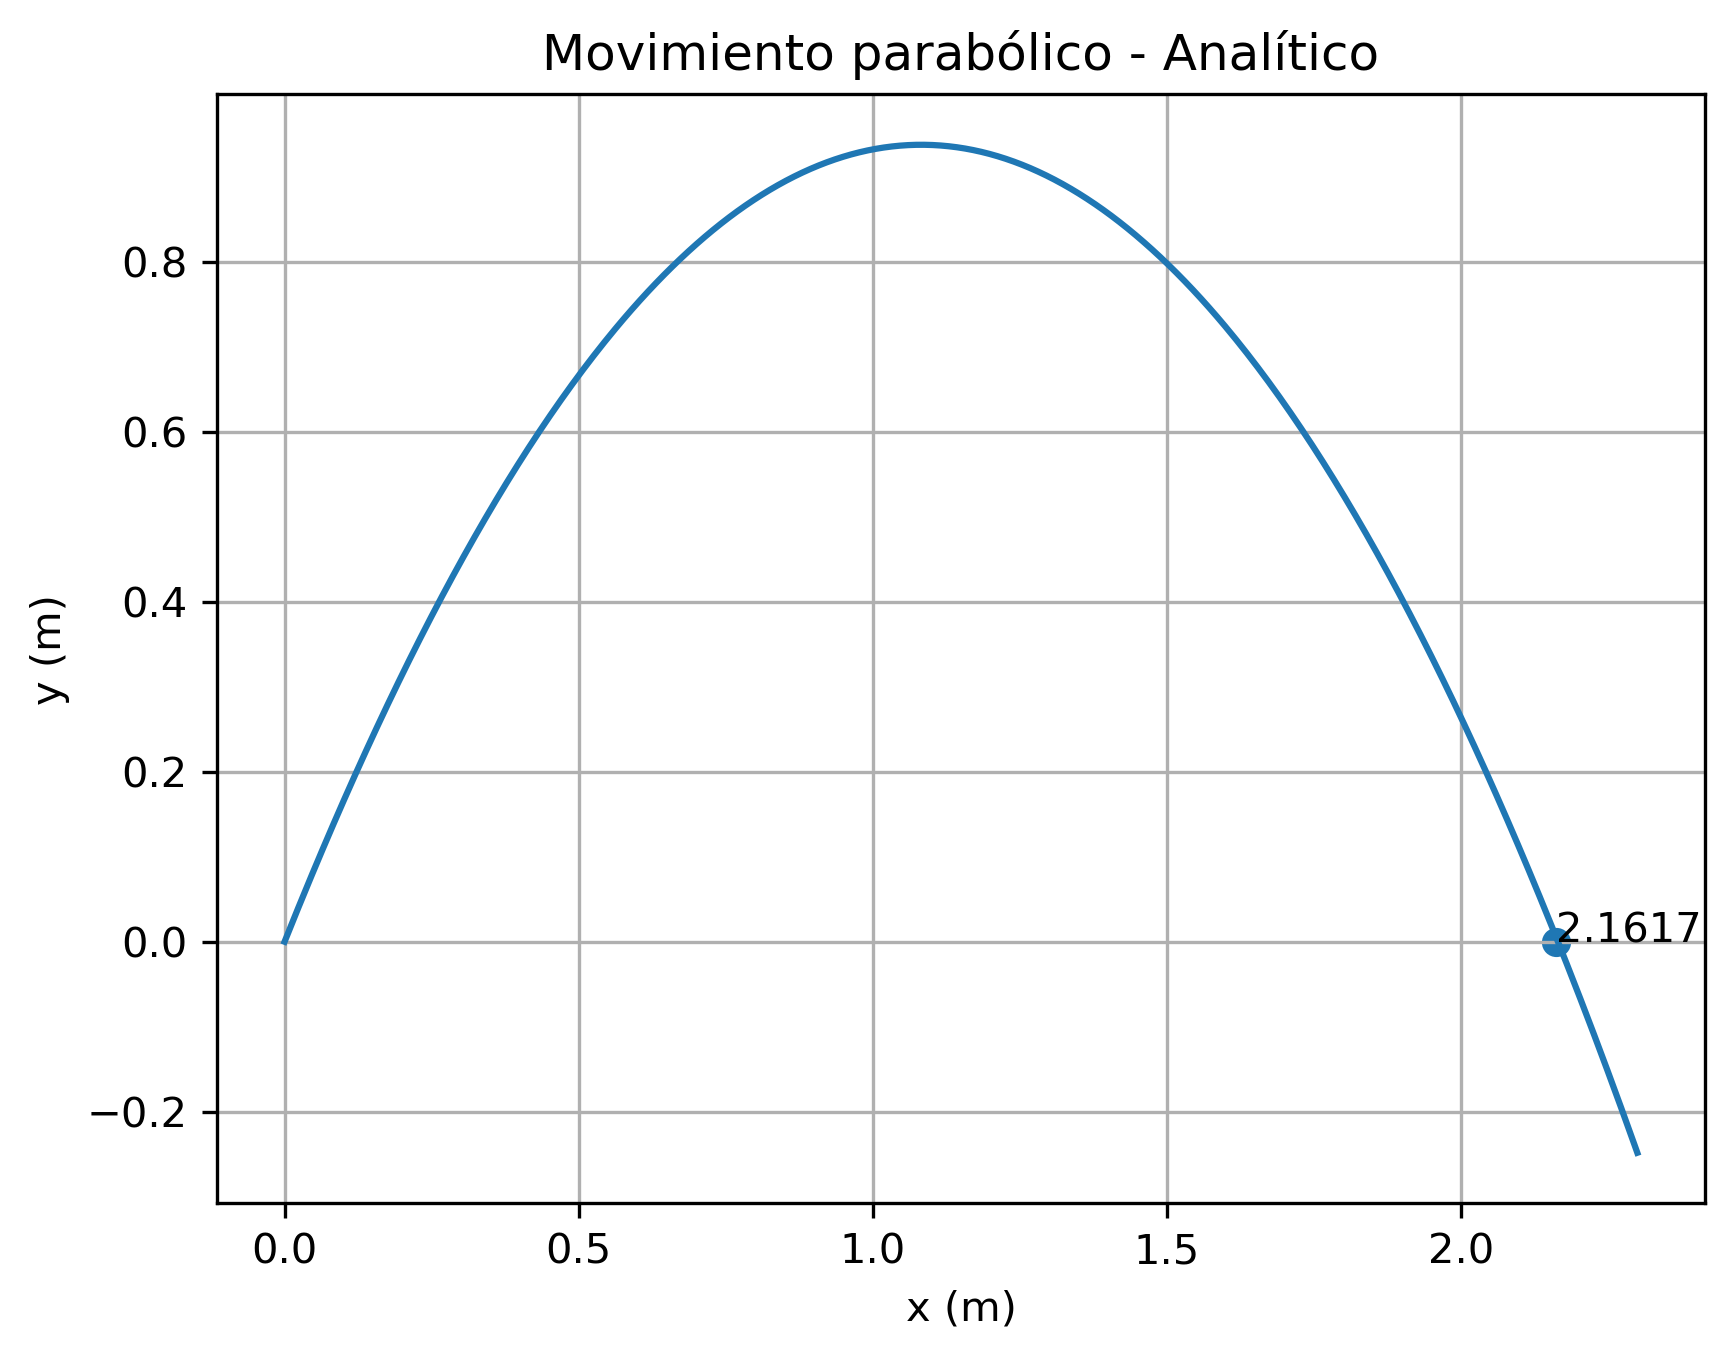
\includegraphics[width=0.7\textwidth]{images/problem01_1.png}
  \caption{Solución analítica.}
  \label{fig:prob1_1}
\end{figure}

A partir de la gráfica obtenida, se observa que el proyectil alcanza aproximadamente una distancia horizontal de $\SI{2.16}{\meter}$ antes de regresar al suelo.

\subsection{Aplicación del método de Heun}

Para resolver numéricamente el movimiento parabólico, se empleó el método de Heun, el cual corresponde a un método predictor-corrector de segundo orden utilizado para aproximar soluciones de ecuaciones diferenciales ordinarias.

El movimiento de la partícula puede describirse mediante el siguiente sistema:

\begin{equation}
    \frac{dx}{dt} = v_x
\end{equation}

\begin{equation}
    \frac{dy}{dt} = v_y
\end{equation}

\begin{equation}
    \frac{dv_x}{dt} = 0
\end{equation}

\begin{equation}
    \frac{dv_y}{dt} = a
\end{equation}

donde la aceleración gravitacional se considera constante:

\begin{equation}
    a = -\SI{10}{\meter/\second^2}
\end{equation}

Las componentes iniciales de la velocidad se calcularon a partir de la velocidad inicial y el ángulo de lanzamiento:

\begin{equation}
    v_{x0} = v_0 \cos \alpha_0
\end{equation}

\begin{equation}
    v_{y0} = v_0 \sin \alpha_0
\end{equation}

El método de Heun se aplicó utilizando un esquema predictor-corrector. En cada iteración, primero se estimó una velocidad vertical predictora mediante el método de Euler y posteriormente se corrigió la posición vertical utilizando el promedio entre la pendiente inicial y la pendiente predicha.

La integración numérica se realizó para intervalos de tiempo separados por un tamaño de paso $h = 0.01$. La simulación continuó hasta que la partícula regresó al suelo, es decir, cuando la coordenada vertical tomó valores menores que cero.

La implementación desarrollada se muestra en el Código \ref{lst:prob1_2}.

\begin{listing}[H]
\inputminted[
  linenos,
  frame=lines,
  mathescape,
  fontsize=\small
]{python}{code/problem01_2.py}
\caption{Implementación del método de Heun para el movimiento parabólico.}
\label{lst:prob1_2}
\end{listing}

La Figura \ref{fig:prob1_2} muestra la trayectoria obtenida mediante el método numérico.

\begin{figure}[H]
  \centering
  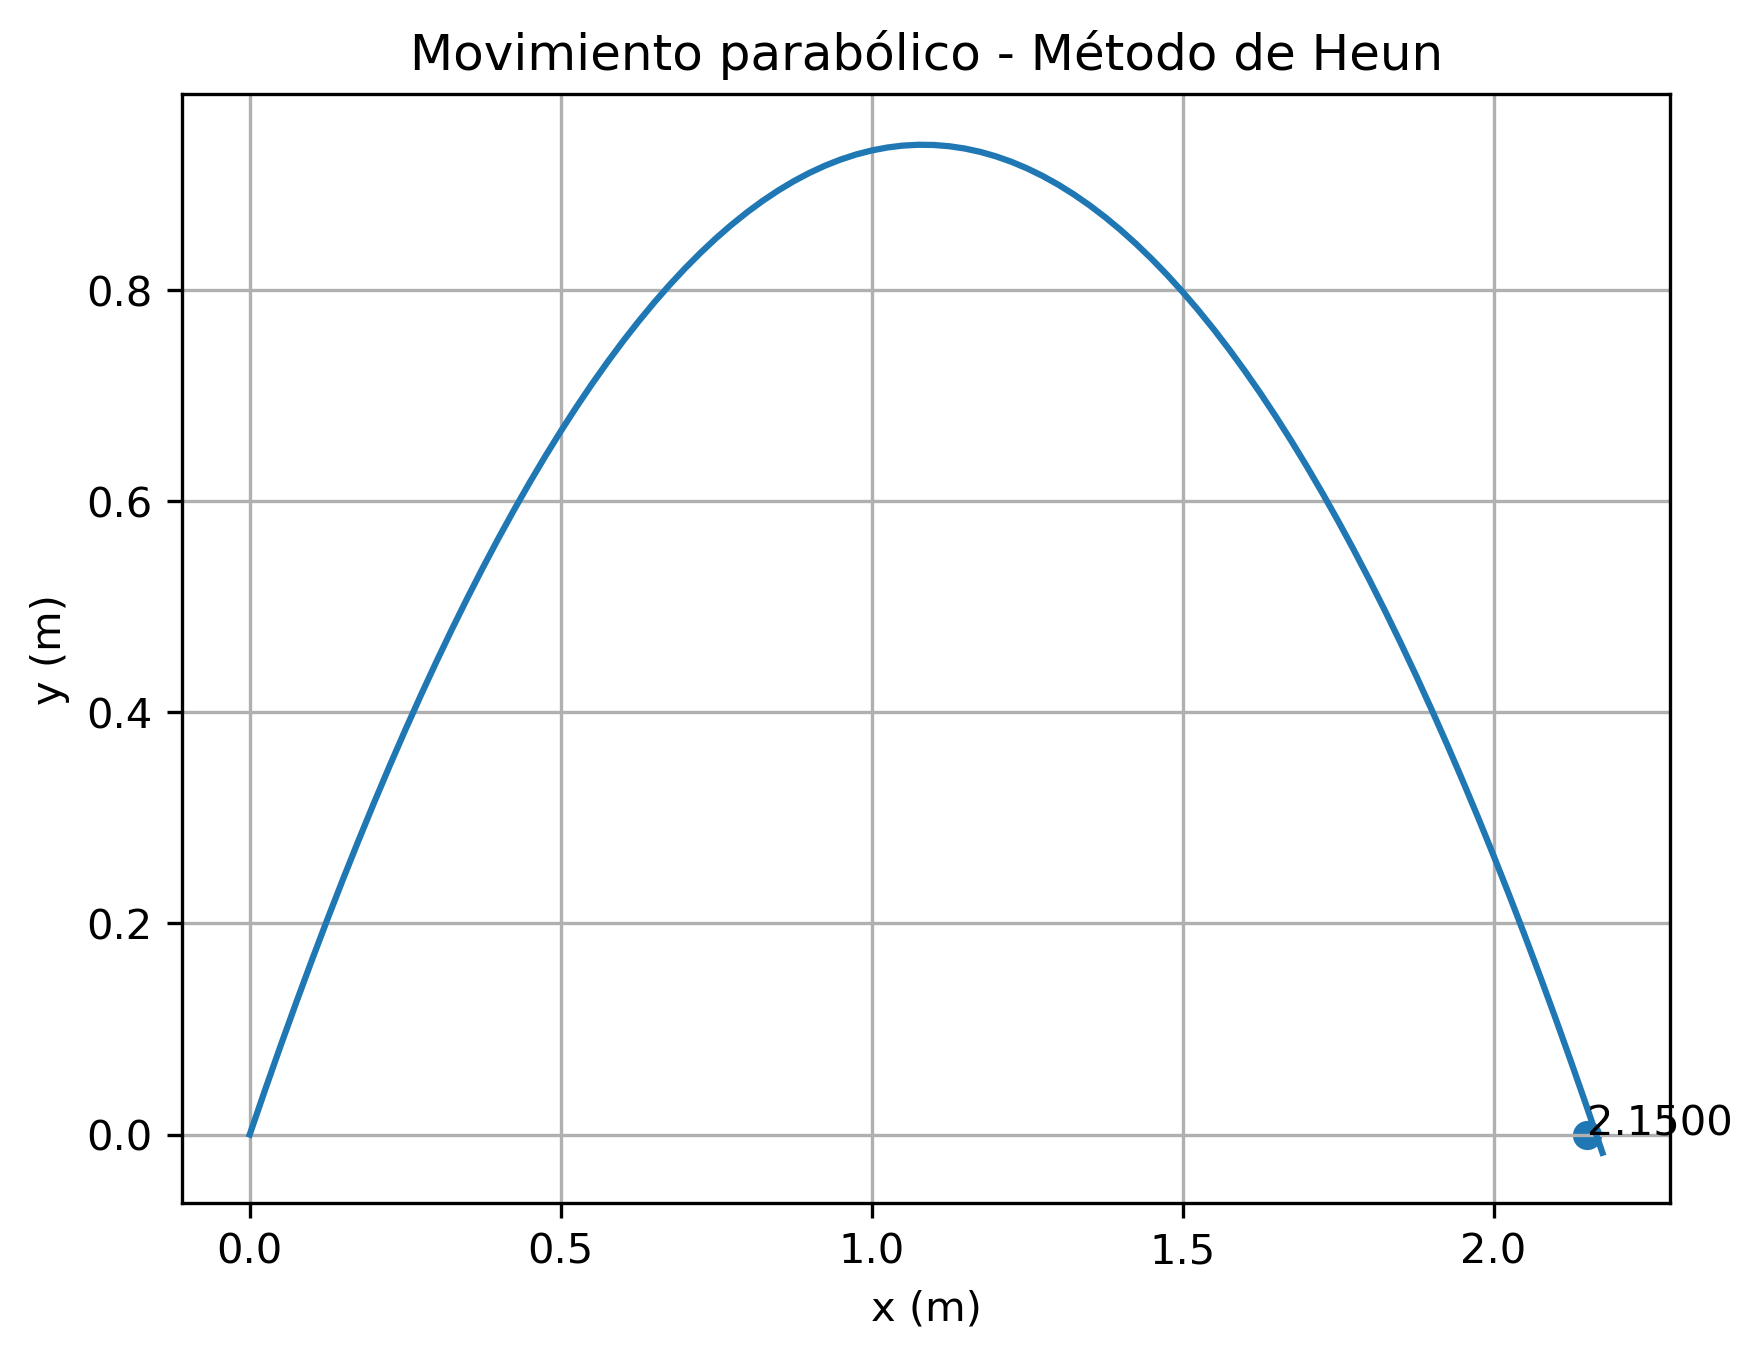
\includegraphics[width=0.7\textwidth]{images/problem01_2.png}
  \caption{Trayectoria obtenida mediante el método de Heun.}
  \label{fig:prob1_2}
\end{figure}

El alcance horizontal obtenido mediante el método de Heun fue aproximadamente $\SI{2.16}{\meter}$, mostrando una buena concordancia con el resultado analítico obtenido previamente.

\subsection{Comparación de resultados}

Finalmente, se realizaron simulaciones utilizando distintos tamaños de paso $h$ con el objetivo de analizar la convergencia del método de Heun. Para cada simulación, el alcance horizontal se determinó tomando el último punto válido antes de que la trayectoria atraviese el suelo, es decir, antes de que la coordenada vertical tome valores negativos.

Posteriormente, los resultados numéricos fueron comparados con el alcance obtenido mediante la solución analítica desarrollada en la primera parte del problema.

Los resultados obtenidos se muestran en la Tabla \ref{tab:comparacion}.

\begin{table}[H]
\centering
\begin{tabular}{ccc}
\hline
Paso $h$ & Alcance obtenido (m) & Error relativo (\%) \\
\hline
0.1   & 2.0000 & 7.4812 \\
0.01  & 2.1500 & 0.5423 \\
0.001 & 2.1650 & 0.1516 \\
\hline
\end{tabular}
\caption{Comparación del alcance para diferentes tamaños de paso.}
\label{tab:comparacion}
\end{table}

Se observa que el alcance calculado mediante el método numérico depende directamente del tamaño de paso utilizado durante la integración temporal. Para valores grandes de $h$, la simulación produce una aproximación menos precisa debido a que el método avanza mediante intervalos discretos relativamente amplios.

Al disminuir el tamaño de paso, los puntos calculados se aproximan progresivamente a la trayectoria analítica y el error relativo disminuye considerablemente. Esto evidencia la convergencia del método de Heun hacia la solución exacta del problema.

En conclusión, el método de Heun proporciona resultados satisfactorios para el movimiento parabólico y mejora su precisión conforme se reduce el tamaño de paso empleado en la simulación.

% \input{sections/problema2}
% \input{sections/problema3}
% \input{sections/problema4}

% References
\newpage
\printbibliography[heading=bibintoc, title={Referencias}]

\end{document}
